\documentclass[a4paper, 12pt]{article}
\usepackage{titling}
\usepackage{array}
\usepackage{booktabs}
\usepackage{enumitem}
\usepackage{graphicx}
\usepackage{hyperref}
\usepackage{amssymb}
%\usepackage{mathtools}
\usepackage{listings}
\usepackage{amsmath}
\usepackage{color} %red, green, blue, yellow, cyan, magenta, black, white
\setlength{\heavyrulewidth}{1.5pt}
\setlength{\abovetopsep}{4pt}
\setlength{\parindent}{0pt}
\graphicspath{{.}}
\usepackage{float}
\usepackage[margin=1in]{geometry}
\definecolor{mygreen}{RGB}{28,172,0} % color values Red, Green, Blue
\definecolor{mylilas}{RGB}{170,55,241}
% Must be after geometry
\usepackage{fancyhdr}
\pagestyle{fancy}
\fancyhf{}
\rhead{NN Homework 9}
\lhead{P.Lukin, E. Ovchinnikova}
\cfoot{\thepage}

\setlength{\droptitle}{-5em}

\title{Neural Networks  \\
				- Homework 9 -}
\author{Petr Lukin, Evgeniya Ovchinnikova}
\date{Lecture date: 21 November 2016}

\begin{document}

%-------------------------------------------------------------------------------
\lstset{language=Matlab,%
    %basicstyle=\color{red},
    breaklines=true,%
    morekeywords={matlab2tikz},
    keywordstyle=\color{blue},%
    morekeywords=[2]{1}, keywordstyle=[2]{\color{black}},
    identifierstyle=\color{black},%
    stringstyle=\color{mylilas},
    commentstyle=\color{mygreen},%
    showstringspaces=false,%without this there will be a symbol in the places where there is a space
    numbers=left,%
    numberstyle={\tiny \color{black}},% size of the numbers
    numbersep=9pt, % this defines how far the numbers are from the text
    emph=[1]{break},emphstyle=[1]\color{red}, %some words to emphasise
    emph=[2]{end,function}, emphstyle=[1]\color{blue},
}

%-------------------------------------------------------------------------------

\maketitle

\section{Mind map}
\begin{figure}[h]
  \centering
  \caption{Mind map. Chapter 9 from Haykin's book. A zoomed version is attached as SOMs.png}
  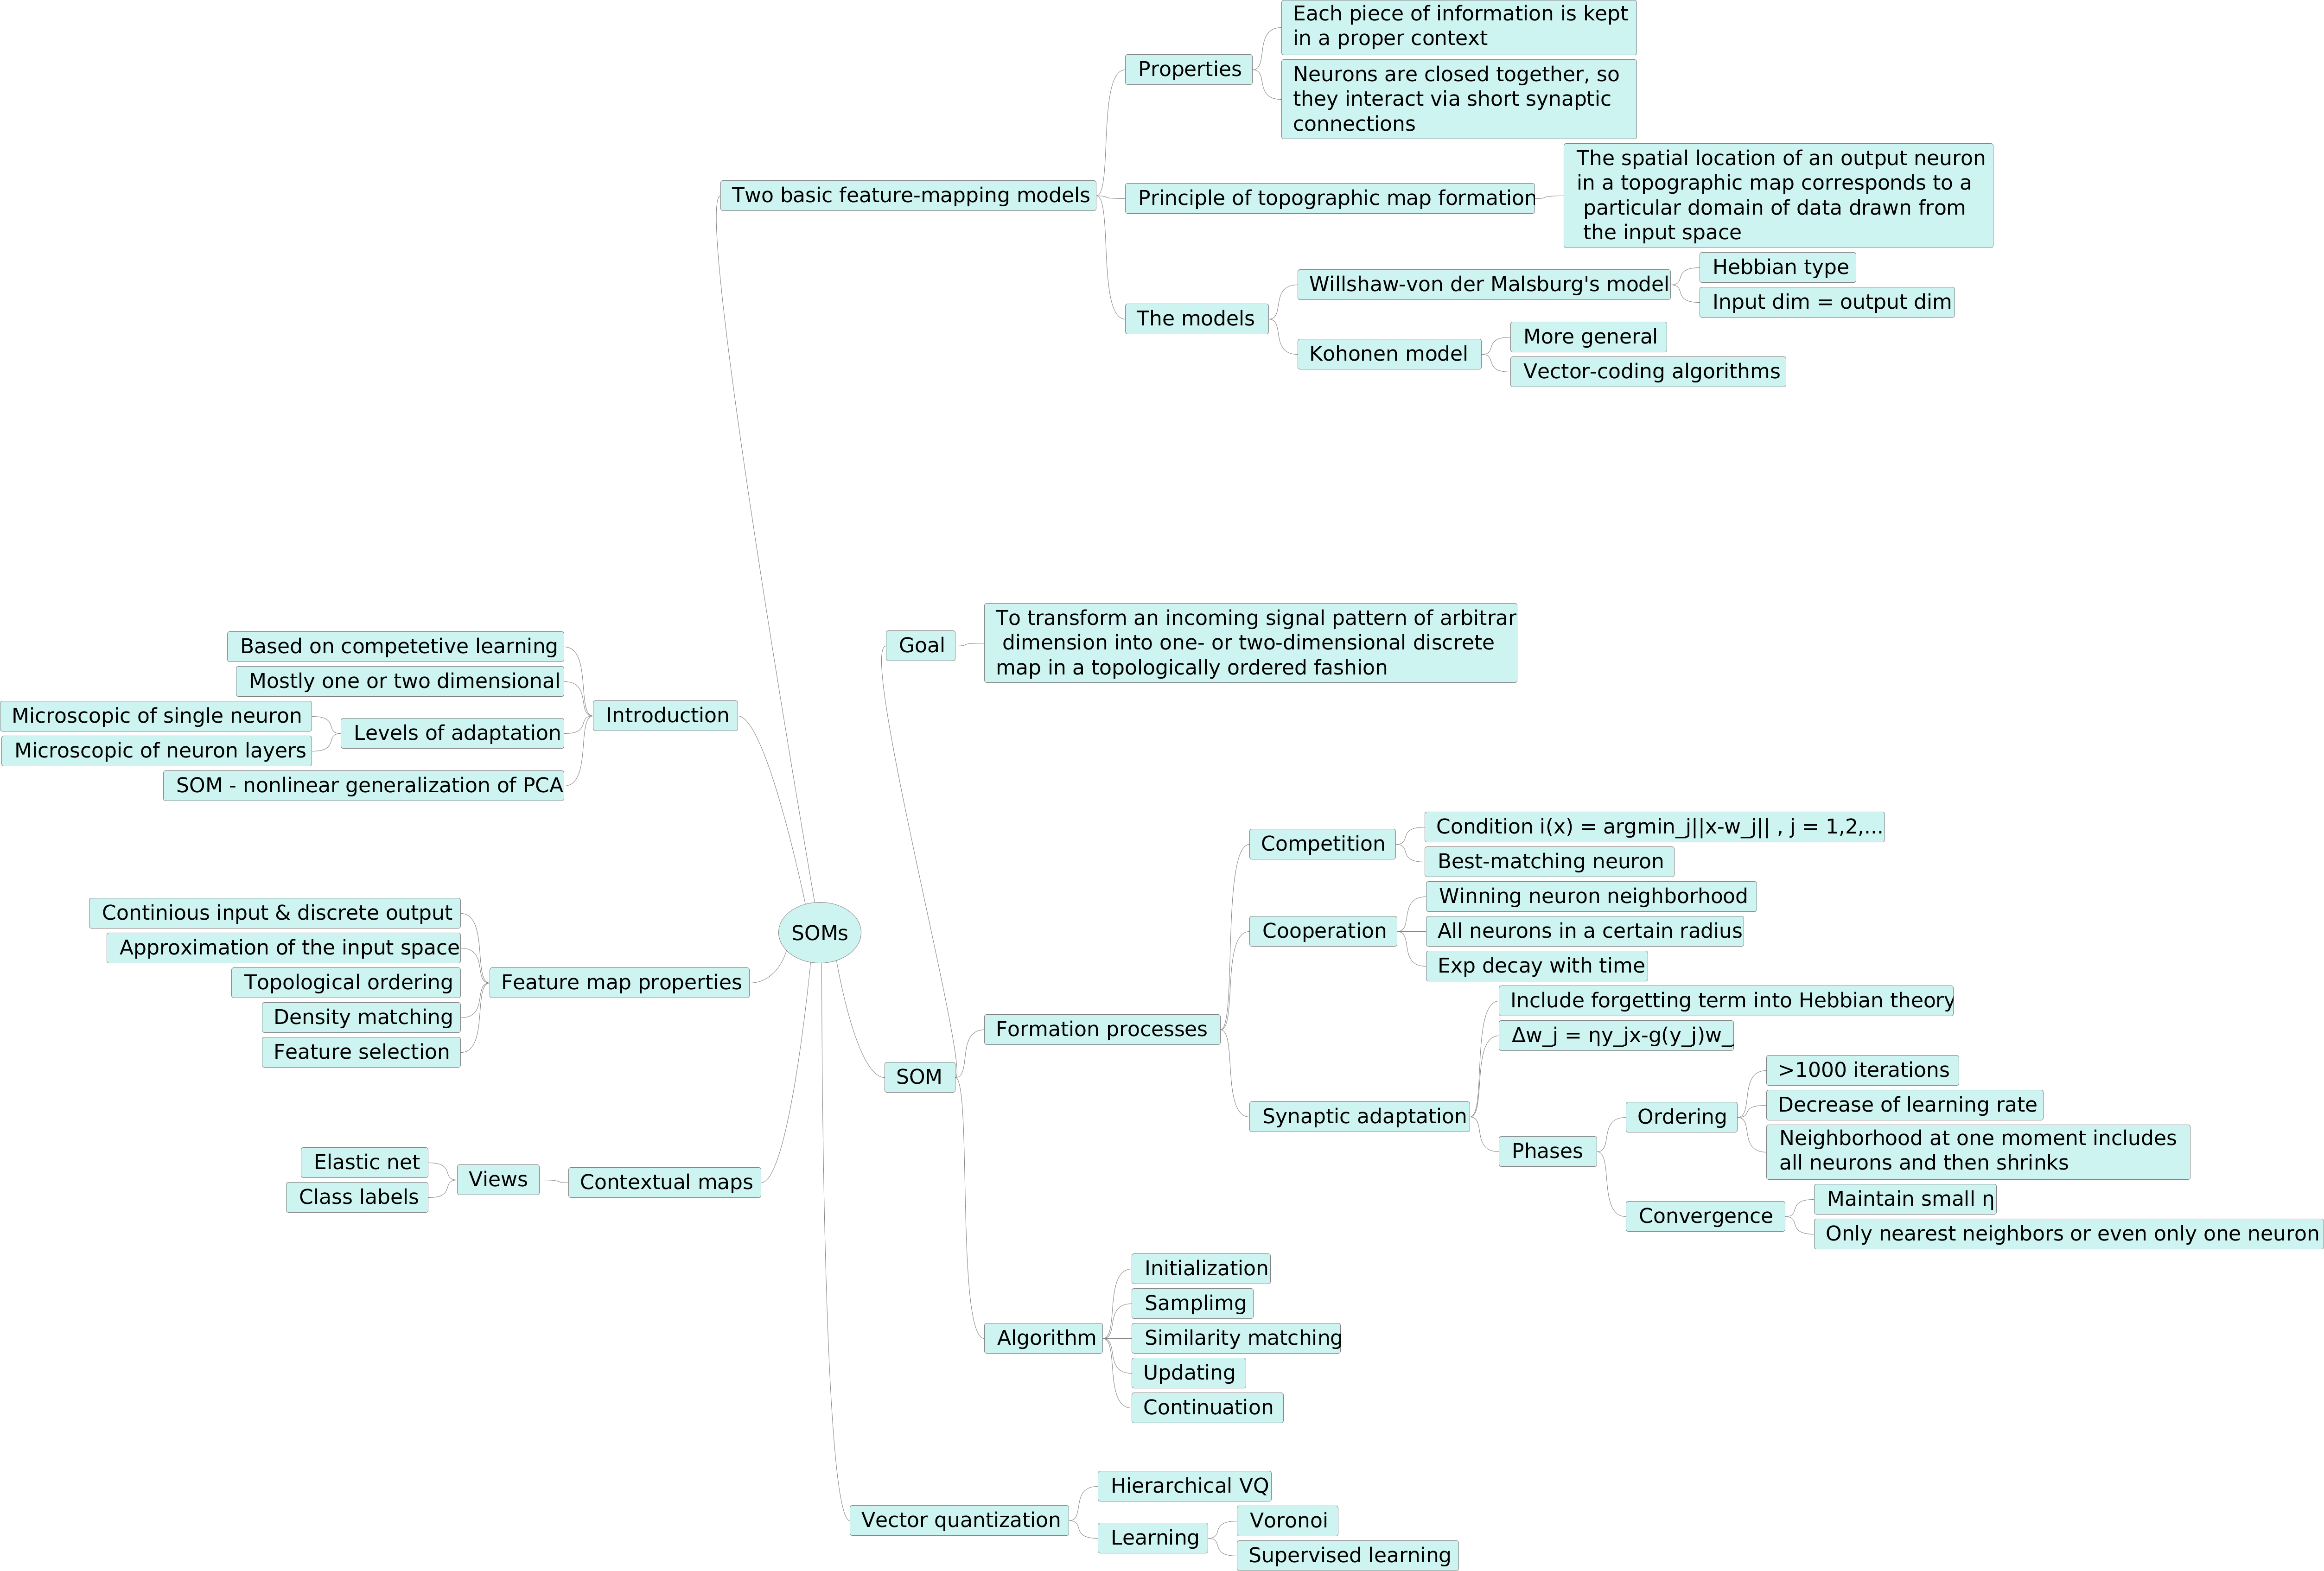
\includegraphics[width=1.0\textwidth]{SOMs}
\end{figure}

\section{Exercises}

\subsection{Exercise 2}
Show that in the SOM algorithm the winner neuron for an input $x$ is the neuron $k$ whose weight vector $w_k$ maximizes the inner product $< w k ,x >$ of x and w k , with $x$ and $w_k$ normalized.

\subsection{Exercise 3}

Consider the one dimensional input space S={0.1, 0.2, 0.4, 0.5}.
Cluster S using a one dimensional SOM network with:

\begin{itemize}
\item 2 nodes.
\item learning rate equal to 0.1.
\item Neighborhood function which is equal to 1 for the winner neuron and is 0 otherwise.
\item Weight initialization:
\begin{itemize}
\item $w_1$=0.15, $w_2$=0.45
\item $w_1$=0.3, $w_2$=0.9
\end{itemize}
\item Stopping criterion: $$\sum_{i=1}^2|w_i^{old} - w_i^{new}| < 0.01$$
\end{itemize}

Comment on the two clusterings you obtained using the two different weight initializations.

\subsection{Exercise 4}
Program a SOM to solve the traveling salesman problem (TSP):
\begin{itemize}
\item  Input layer contains just two neurons called "Xcoord" and "Ycoord"
\item The Kohonen lattice is thought of as a circle containing at least as many neurons as we have cities (usage of more neurons is possible), the neurons are numbered in round about fashion.
\item Each neuron n(i) (numbered by i) on the circle is connected to "Xcoord" and "Ycoord" and the weights on these edges are the initial x and y coordinates of the neuron in the plane (see picture)
\item The input patterns are the (x,y) coordinates of all target cities.
\item When applying one concrete city pattern the winner is of course the neuron with lies closest to the given city. Only the weights of the winning neuron will be adapted according to the learning rule, no other neighboring weights are changed. This "moves" the neuron closer to "its" city.
\item After some cycles there is just ONE neuron closest to each city. These build pairs (n(i),City(closest to n(i)).
\item If we sort this pairs according to the number of the neurons "i" this will give a journey for the respective cities, which solves the TSP approximately. 
\item Use tools like ICONNECT, TSPLIB or alike to do the programming, compare runtime, memory and achieved length of path.

\end{itemize}


\lstset{language=Python}
\begin{lstlisting}[frame=single]

\end{lstlisting}


\end{document}
